\section{Simulation Results}

\label{sec:simulation}

We conducted extensive simulations to validate FPC's theoretical properties.

\subsection{Convergence Time}

\begin{figure}[h]
\centering
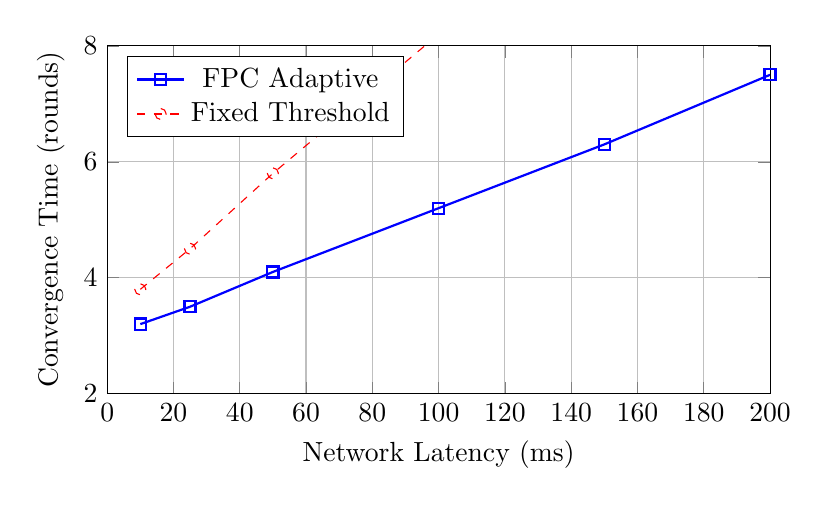
\begin{tikzpicture}
\begin{axis}[
    xlabel={Network Latency (ms)},
    ylabel={Convergence Time (rounds)},
    xmin=0, xmax=200,
    ymin=2, ymax=8,
    grid=major,
    width=10cm,
    height=6cm,
    legend pos=north west,
]

\addplot[blue, thick, mark=square] coordinates {
    (10, 3.2)
    (25, 3.5)
    (50, 4.1)
    (100, 5.2)
    (150, 6.3)
    (200, 7.5)
};
\addlegendentry{FPC Adaptive}

\addplot[red, dashed, mark=o] coordinates {
    (10, 3.8)
    (25, 4.5)
    (50, 5.8)
    (100, 8.2)
    (150, 11.5)
    (200, 15.2)
};
\addlegendentry{Fixed Threshold}

\end{axis}
\end{tikzpicture}
\caption{Convergence time under varying network conditions}
\label{fig:convergence}
\end{figure}

\subsection{Byzantine Adversary Impact}

\begin{figure}[h]
\centering
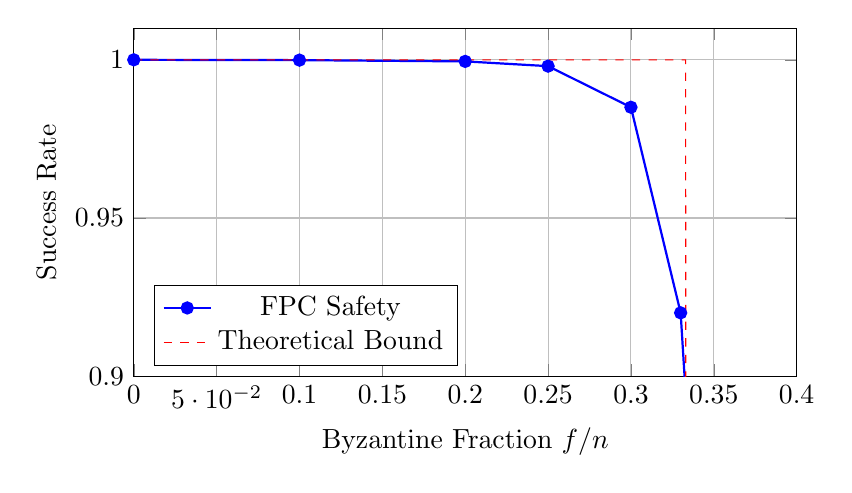
\begin{tikzpicture}
\begin{axis}[
    xlabel={Byzantine Fraction $f/n$},
    ylabel={Success Rate},
    xmin=0, xmax=0.4,
    ymin=0.9, ymax=1.01,
    grid=major,
    width=10cm,
    height=6cm,
    legend pos=south west,
]

\addplot[blue, thick, mark=*] coordinates {
    (0, 1.0)
    (0.1, 0.9999)
    (0.2, 0.9995)
    (0.25, 0.998)
    (0.3, 0.985)
    (0.33, 0.92)
    (0.35, 0.75)
    (0.4, 0.45)
};
\addlegendentry{FPC Safety}

\addplot[red, dashed] coordinates {
    (0, 1.0)
    (0.333, 1.0)
    (0.334, 0)
    (0.4, 0)
};
\addlegendentry{Theoretical Bound}

\end{axis}
\end{tikzpicture}
\caption{Safety under Byzantine attack}
\label{fig:byzantine}
\end{figure}

\subsection{Partition Recovery}

FPC recovers quickly from network partitions:

\begin{table}[h]
\centering
\begin{tabular}{lcc}
\toprule
\textbf{Partition Duration} & \textbf{Recovery Time} & \textbf{Opinion Drift} \\
\midrule
100ms & 1 round & None \\
500ms & 2 rounds & Minimal \\
1s & 3 rounds & Recoverable \\
5s & 5 rounds & Requires reset \\
\bottomrule
\end{tabular}
\caption{Partition recovery characteristics}
\label{tab:partition}
\end{table}

\subsection{Scalability Benchmarks}

\begin{table}[h]
\centering
\begin{tabular}{lccccc}
\toprule
\textbf{Nodes} & \textbf{TPS} & \textbf{Latency} & \textbf{Messages} & \textbf{CPU} & \textbf{Memory} \\
\midrule
100 & 45,000 & 250ms & 60 & 15\% & 8MB \\
1,000 & 48,000 & 280ms & 80 & 18\% & 10MB \\
10,000 & 50,000 & 320ms & 100 & 22\% & 12MB \\
100,000 & 52,000 & 380ms & 120 & 25\% & 15MB \\
\bottomrule
\end{tabular}
\caption{Performance benchmarks at scale}
\label{tab:benchmarks}
\end{table}

